\documentclass[11pt,a4paper]{article}
\usepackage{a4wide,url,graphicx}
\usepackage[utf8]{inputenc}
\usepackage[english]{babel}

\newcommand{\ccnotice}{\vfill
  \begin{minipage}{.22\textwidth}\centering
    \includegraphics[width=\textwidth]{by.png}
  \end{minipage}\hfill\begin{minipage}{.77\textwidth}
  This text can be reused under the terms of the Creative Commons CC-BY
  License \url{https://creativecommons.org/licenses/by/3.0}.
  \end{minipage}
}

\parindent0pt
\parskip4pt
\title{Handout for a Seminar Paper \\[4pt] on the topic \emph{Patent Search}}

\author{Hans-Gert Gr\"abe, Leipzig}
\date{July 24, 2019}

\begin{document}
\maketitle

\section{General}

In the seminar paper on the topic \emph{patent search} five selected patent
documents are to be analysed to trace Altschuller's way to his basic
structural statements about the creative process in the engineering invention
process.

The core of the approach is the transition from a \emph{special problem} to a
\emph{special solution} (as described in the patent) as an abstraction
process, that
\begin{itemize}
\item assigns the specific problem to a general problem class,
\item suggests solutions to the general problem from analogy considerations   
\item and finally breaks down these solutions to a special solution of the
  special problem.
\end{itemize}
\begin{center}
  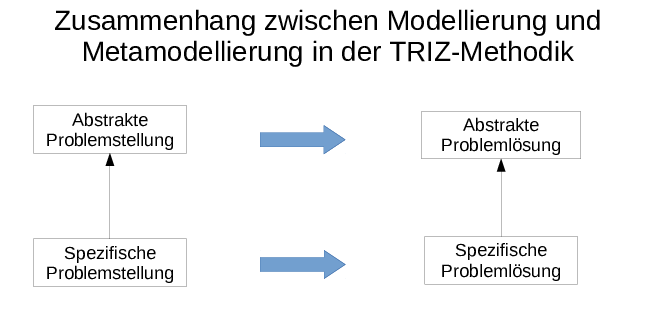
\includegraphics[width=.7\textwidth]{2019-04-25/Folie-1.png}
\end{center}
In contrast to Altshuller's beginnings, today exist elaborated,
experience-based TRIZ tools and concepts to propose solutions to the general
problem.

The aim of the analysis of the patent specification is to determine the
suitability of this general principles on the context of the specific solution
of the specific problem described in the patent claim. For this, first the
specific problem and the specific solution are to be extracted in sufficiently
general and meaningful terms.  Based on such a description the specific
solution process has to be related to appropriate more general TRIZ
principles, wherein the elaboration of a \emph{main contradiction} in the
specific problem definition has a guiding function.

Such a contradiction always exists only \emph{relative to the state of the
  art}\footnote{German: „Stand der Technik“.}, since it is the goal of the
various TRIZ principles, to resolve such contradictions and thus to define a
\emph{new state of the art}, in which the solution strategies for \emph{this}
contradiction have become commonplace. So it is important to describe the
respective state of the art, against which the further argumentation is
performes. The \emph{state of the art} assumed to be known to a „skilled
person“ is always a temporal relative phenomenon. On the contrary, TRIZ
studies teh deveolopment of historical ideas.

In some cases, such a major contradiction may be difficult identify. Here it
would be necessary to investigate if the patented solution is a \emph{standard
  solution} by a non-obvious parameter optimization is. This is often an
indication that the modeling of the context goes too far and the resolution of
the contradiction is already subsumed within the state of the art.

Therefore to process the patent analysis the following steps required:
\begin{itemize}
\item [1.] Extract the patent metadata.
  
\item [2.] Describe the state of the art with respect to the problem setting.

  A patent must always have a \emph{inventiveness} level compared to the state
  of the art, that is not obvious to a skilled person. The patent claim to be
  described is understandable only in such a context of previous technical
  developments, that are known to a skilled person, but not to the readers of
  the seminar work. This context of historical development of ideas (that is
  important also to recognize for the TRIZ analysis) must therefore first
  \emph{sufficiently accurate} to be described.

\item [3.] Description of the functional model.

  After marking this context, it is necessary to explain the concepts in more
  detail that are relevant to describe the problem and solution presented in
  the patent claim.

  For this purpose, first the system has to be delimited within a super
  system.  Often a system fulfills a specific function within such a super
  system that needs to be worked out at this point.
  
  For this, the \emph{Innovation Checklist} [KS: Chap. 5.1] may be a good
  guidamce. Furthermore, it can be useful to identify
  \begin{itemize}
  \item functions -- main function(s), secondary functions [KS: Chap. 4.1.]
    and
  \item resources -- type, properties, behavior [KS: Chap. 4.2]
  \end{itemize}
  within the system.

\item [4.] Formulation of the \emph{miniproblem}: elaboration of the basic
  problem as \emph{special problem} formulation a contradiction.

\item [5.] Description of the solution to the problem in the patent claim as
  \emph{special solution}.

\item [6.] Classification of the problem in the TRIZ classification as
  \emph{general problem}.

\item [7.] Description of the relation of the special solution to the general
  TRIZ structures.
\end{itemize}

This methodology is prototypically described in the following example.

\section{Example: Patent EP0066122B1}

\subsection{metadata}
\begin{itemize} \itemsep0pt
\item Title: Differential gearings
\item Source: \url{https://patents.google.com/patent/EP0066122B1}
\item Patentee: Theodoros Tsiriggakis
\item Patent Data: publication 1982-12-08, notice of the Patent Grant
  1985-05-15
\item Classification by Google:
  \begin{itemize}
  \item F16 H 48/147 Differential gearings without gears with driven cam
    followers or balls engaging two opposite cams
  \end{itemize}
\end{itemize}

\subsection{Description of the State of the Art}

When a vehicle drives through a bend, the outer wheels put one further way
than the inner ones and therefore have to turn faster.  For this purpose, the
rotational speed of the drive axle has to be adjusted during transfer to the
driven shafts with different, adapted to the particular driving situation
ratios.

This is usually done with a differential gearing on the basis of gears. The
two driven shafts sit on a common axle, are sprockets mounted and
interconnected through one or more pinions. These pinions convey the
differential speed between both shafts. The drive energy can be conducted
directly to one of the two shafts or via a crown wheel of various ways into
the gear design, such as comparable to this patent -- by fixing the pinion
with the crown wheel are connected. In this case, over the pinion not only the
speed ​​compensation mediated, but also the power transmission. More detailed
explanations can be found in the Wikipedia [DG].

In the class F16H48 of the [IPC], patents become different versions detected
such differential gear. In a class of Differential gears are used instead of a
pinion rolling elements to the Speed ​​compensation between two plates to get on
the driven shafts are mounted. This principle was created in 1932 by Andrew
Francis Ford patented (patent US1897555) and is in the present Patent document
referred to as a „generic city of technology“, which also as patent class
F16H48 / 147 in the [IPC]. So it can be like that be assumed that even at the
time of filing the patent this basic type of execution of a differential gear
for „Stand the technique“ belonged.

As previous problems are mainly friction losses of the rolling elements
listed, which lead to restless running and rapid wear. Furthermore can in
conventional Ausführung a differential gear on black ice spin one wheel at
double speed while the other one stationary.

\subsection{Functional Model}

\paragraph{Supersystem.}
Entry of rotational energy via the drive shaft, transmission of Rotational
energy on the two driven shafts while adjusting the Speed ​​to drive the wheels
accordingly.

\paragraph{Components.}
\begin{itemize}
\item \emph{Powered Waves} -- Waves connected to the wheels, the on a common
  axis, the \emph{system axis}, are mounted.
\item \emph{transmission element}, \emph{gear carrier} (also cage or Basket)
  -- entry of the drive power into the system via the driving Wave, relative
  to which the speed of the two driven Waves must be adjusted. In the patent
  specification as \emph{crown wheel} executed, which is parallel to the cam
  track plates, so that a fixed Connection between crown gear and cam track
  plates a uniform Rotary motion would lead to the driven axles.
\item \emph{cam track} -- concentric with the axis of the cam track plate
  executed guide structure for the rolling elements on the cam track plate,
  over which the movement of the rolling elements is controlled. A rolling
  element lies on the corresponding cam tracks of the opposite Cam track plate
  and rotates with the differential speed of driven wheels.
\item \emph{cam plate} -- transmission unit of movement on one of the driven
  waves. With a splined shaft is achieved that the cam track plates can move
  in the direction of the system axis.  The required back-adjusting force by a
  spring, which the Cam plate pressed against the rolling elements, is not
  listed and heard probably the state of the art.
\item \emph{system axis} -- common axis of rotation of the cam track plates
  and the Face gear.
\item \emph{rolling elements} -- complex in this patent Transmission element
  for speed adaptation and simultaneous Power transmission from the crown
  wheel to the cam track plates and further to each the two driven waves.
\end{itemize}

\paragraph{How the system works:}
From the drive shaft, the rotation is rigid on the crown wheel and on transmit
the Wälzkörperstruktur fixed in the crown wheel, which the Rotary movement via
the cam structures on the two cam track plates transferred and by
corresponding self-rotating movements at the same time for the Velocity
compensation according to the over the driven shafts ensure registered speed
differences.

The rolling elements are fixed in „cage structures“ on the crown wheel such
that they move with the crown wheel and both the power transfer as also the
speed compensation to the cam track plates only by can convey limited
movements relative to the crown wheel. The Rolling elements can move
perpendicular to the direction of rotation of the crown wheel as well as
turning around its own axis.
  
\subsection{Formulation of the Miniproblem}

For good grip (power transmission), the rolling elements must be as strong as
possible with the Cam track plates connected, for the compensation of the
speeds they must roll freely on the cam tracks.

The rolling elements should turn so (for speed compensation) and Do not turn
(for power over) at the same time.

In the Ritzellösung spinning is in the foreground, which is why it under
extreme operating conditions for spinning a wheel at the same time Standstill
of the other wheel can come.

\subsection{Description of the solution to the problem in the patent
  specification} 

By a sinusoidal design of the cam tracks -- in the minima is the Grip
particularly high, since the potential energy is minimized in the Maxima, the
rolling motion is particularly favorable, since there is no Potential
resistance is overcome -- alternate layers with high Power transmission and
layers with low rolling resistance.

By the execution of two cam tracks, which are twisted against each other, is
achieved that the rolling elements are on a track in the minimum and thus give
maximum grip when the rolling elements on the other track the Go through
maximum.

Rolling elements carry both straight-line movements (perpendicular to the
plane of rotation, according to the state on the cam track) as well as
rotational movements. The vertical displacement movements are by the two cam
tracks phased out, the rotational movements by that of the driven Axes
transmitted speed differential. Both movements show different friction
behavior. Through a layer structure of Rolling element is achieved that in the
first layer, the „linear guide“ along the system axis in a V-shaped groove and
in the second layer the „Drehlagerung“ is executed in a conical recess. The
Total movement is thus separated into these two movements to those for the to
realize each movement most advantageous structural form.

The cam track plates are symmetrical to each other, which is a enables
particularly simple production.

The cam track plates transmit the same torque in the basic position the axles
and slip in at a difference in the speeds repeatedly in this basic position,
so that the above-described „black ice effect“ not can occur.

\subsection{Classification of the problem in the TRIZ systematics}

The solution does not work directly into the \emph{contradiction matrix
  Altschuller}, because here the power transmission and the rolling resistance
in conflict with each other.

In the \emph{contradiction matrix 2003} the problem can only be roughly
explained as Classify conflict between power and speed, of the four Proposals
is only the principle of dynamization implemented.

Overall, the solution has more of the character of a further optimized, im
Principle already found solution (design of the cam track, more accurate
structure the rolling elements).

\subsection{Representation of the reference of the special solution to the
  TRIZ structures}

The solution is made by dynamization as well as spatial separation on both the
cam track as well as in the structure of the rolling elements.

Due to the sinusoidal design (odp:P19, principle of the periodic effect)
Change areas with good grip (minima) of rolling bodies with areas better role
property (odp:P15, principle of dynamization).

Due to the division of the rolling elements whose complex movement in one
separated by a linear and a rotary motion, separated for both to enable
optimal constructive solutions (odp:P01, Principle of Decomposition).

Due to the division into two cam tracks offset by $45^\circ$ (odp:P01,
Principle of decomposition) is also achieved that rolling elements always in
the Area with good grip and so on are sufficient power transmission
\emph{both} driven waves is always guaranteed.

Already integrated in the prior art is the concentration of two Functions
(speed compensation and power transmission) in the rolling elements (odp:P06,
principle of universality), the cage structure, about the crown wheel and
rolling elements are connected to each other (odp:P07, principle of Nesting),
as well as the rotationally symmetrical design of the rolling elements
(odp:P14, principle of the ball similarity) as well as the use of Rolling
elements (odp:P24, principle of the mediator).

\section{Literature}
\raggedright
\begin{itemize}
\item{[DG]} Wikipedia entry „Differentialgetriebe“ (differential
  transmission).  \url{https://de.wikipedia.org/wiki/Differentialgetriebe}
  (20.07.2019).
\item{[IPC]} International Patent Classification.
  \url{https://www.wipo.int/classifications/ipc/ipcpub} (20.07.2019).
\item{[KS]} Karl Koltze, Valeri Souchkov: Systematische Innovation (Systematic
  Innovation). 2nd, revised edition Hanser Verlag, Munich 2017.
\item{[PS]} Patent EP0066122B1, published on 15.05.1985 by the
  European Patent Office.
\item{[ZH]} Dietmar Zobel, Rainer Hartmann: Erfindungsmuster (Invention
  Pattern). 2nd, revised edition, Expert Verlag, Renningen 2016.
\end{itemize}

\vfill
\ccnotice
\end{document}
